\documentclass{llncs}
\usepackage{amssymb}
\usepackage{color}
\usepackage{pgf,pgfarrows,pgfnodes,pgfautomata,pgfheaps,pgfshade}
\usepackage{tikz}
\usetikzlibrary{arrows,decorations.pathmorphing,backgrounds,positioning,fit,petri}
\usepackage{amsmath}

\begin{document}

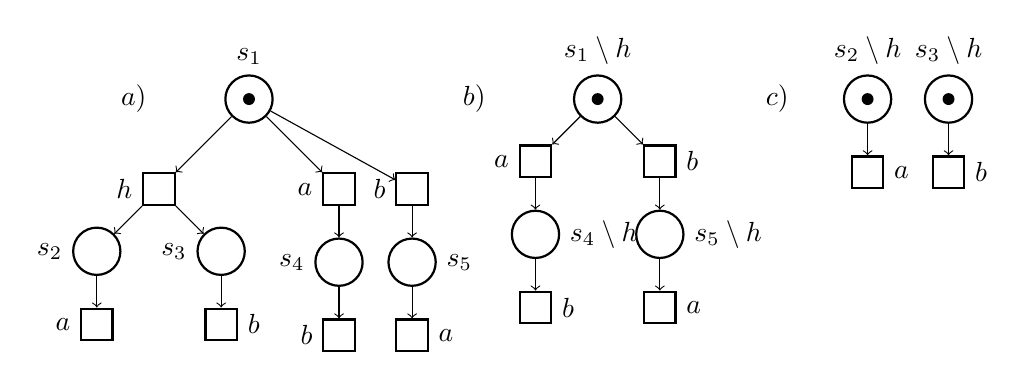
\begin{tikzpicture}[
every place/.style={draw,thick,inner sep=0pt,minimum size=6mm},
every transition/.style={draw,thick,inner sep=0pt,minimum size=4mm},
bend angle=45,
pre/.style={<-,shorten <=1pt,>=stealth,semithick},
post/.style={->,shorten >=1pt,>=stealth,semithick}
]
\def\eofigdist{3.8cm}
\def\eofigdisty{2.8cm}
\def\eodist{0.4}
\def\eodisty{0.5}
\def\eodistw{1}

\node (a) [label=left:$a)\qquad \quad $]{};

\node (q1) [place,tokens=1] [label={above:$s_1$} ] {};
\node (t1) [transition] [below left=\eodistw of q1,label=left:$h$] {};
\node (t2) [transition] [below right=\eodistw of q1,label=left:$a$] {};
\node (t3) [transition] [right=\eodisty of t2,label=left:$b$] {};
\node (q2) [place] [below left=\eodisty of t1,label=left:$s_2$] {};
\node (q3) [place] [below right=\eodisty of t1,label=left:$s_3$] {};
\node (q4) [place] [below=\eodist of t2,label=left:$s_4$] {};
\node (q5) [place] [below=\eodist of t3,label=right:$s_5$] {};
\node (t4) [transition] [below =\eodist of q2,label=left:$a$] {};
\node (t5) [transition] [below =\eodist of q3,label=right:$b$] {};
\node (t6) [transition] [below =\eodist of q4,label=left:$b$] {};
\node (t7) [transition] [below =\eodist of q5,label=right:$a$] {};



\draw  [->] (q1) to (t1);
\draw  [->] (q1) to (t2);
\draw  [->] (q1) to (t3);
\draw  [->] (t1) to (q2);
\draw  [->] (t1) to (q3);
\draw  [->] (t2) to (q4);
\draw  [->] (t3) to (q5);
\draw  [->] (q2) to (t4);
\draw  [->] (q3) to (t5);
\draw  [->] (q4) to (t6);
\draw  [->] (q5) to (t7);


% seconda rete

 
\node (b) [right={3.2cm} of a, label=left:$b)\;\;$] {};

\node (p1) [place,tokens=1]  [right=\eofigdist of q1,label=above:$s_1 \setminus h$] {};
\node (s2) [transition] [below left=\eodisty of p1,label=left:$a$] {};
\node (s3) [transition] [below right=\eodisty of p1,label=right:$b$] {};
\node (p4) [place] [below=\eodist of s2,label=right:$s_4 \setminus h$] {};
\node (p5) [place] [below=\eodist of s3,label=right:$s_5 \setminus h$] {};
\node (s4) [transition] [below =\eodist of p4,label=right:$b$] {};
\node (s5) [transition] [below =\eodist of p5,label=right:$a$] {};

\draw  [->] (p1) to (s2);
\draw  [->] (p1) to (s3);
\draw  [->] (s2) to (p4);
\draw  [->] (s3) to (p5);
\draw  [->] (p4) to (s4);
\draw  [->] (p5) to (s5);







% terza rete
  
 
\node (c) [right={3.6cm} of b,label=left:$c)\;\;$] {};

\node (r2) [place, tokens=1]  [right=\eofigdisty of p1,label=above:$s_2 \setminus h$] {};
\node (r3) [place, tokens=1]  [right=\eodist of r2,label=above:$s_3 \setminus h$] {};
\node (v3)  [transition] [below=\eodist of r2,label=right:$a$] {};
\node (v4)  [transition] [below=\eodist of r3,label=right:$b$] {};

\draw  [->] (r2) to (v3);
\draw  [->] (r3) to (v4);

\end{tikzpicture}

\end{document}